% 2006_sichuan_liberal_q20_fig1: long cuboid with E,P,M,N; schematic projection from original PNG
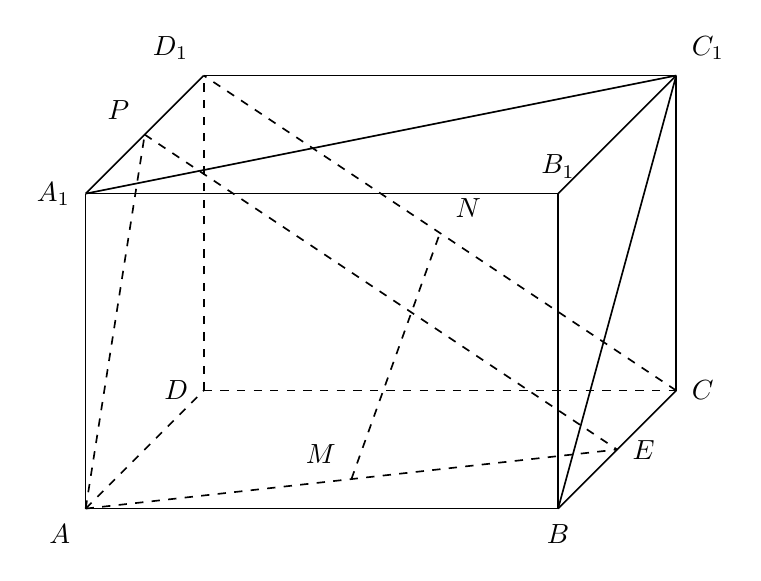
\begin{tikzpicture}[x=1cm,y=1cm,font=\normalsize,line width=.6pt]
\coordinate (A) at (0,0);
\coordinate (B) at (6,0);
\coordinate (C) at (7.5,1.5);
\coordinate (D) at (1.5,1.5);
\coordinate (A1) at (0,4);
\coordinate (B1) at (6,4);
\coordinate (D1) at (1.5,5.5);
\coordinate (C1) at (7.5,5.5);
\coordinate (E) at (6.75,0.75);
\coordinate (P) at (0.75,4.75);
\coordinate (M) at (3.375,0.375);
\coordinate (N) at (4.5,3.5);
% front face solid
\draw[solid] (A) -- (B);
\draw[solid] (B) -- (B1);
\draw[solid] (B1) -- (A1);
\draw[solid] (A1) -- (A);
% depth / top
\draw[solid] (B) -- (C);
\draw[solid] (C) -- (C1);
\draw[solid] (C1) -- (D1);
\draw[solid] (D1) -- (A1);
\draw[solid] (B1) -- (C1);
% hidden base / vertical
\draw[dashed] (A) -- (D);
\draw[dashed] (D) -- (C);
\draw[dashed] (D) -- (D1);
% auxiliary segments visible in original (all dashed except two solid)
\draw[dashed] (A) -- (E);
\draw[dashed] (A) -- (P);
\draw[dashed] (P)--(E);
\draw[solid] (A1) -- (C1);
\draw[solid] (B) -- (C1);
\draw[dashed] (M) -- (N);
\draw[dashed] (C)--(D1);
% labels
\node[below left=2pt] at (A) {$A$};
\node[below=2pt] at (B) {$B$};
\node[right=2pt] at (C) {$C$};
\node[left=2pt] at (D) {$D$};
\node[left=2pt] at (A1) {$A_{1}$};
\node[above=2pt] at (B1) {$B_{1}$};
\node[above left=2pt] at (D1) {$D_{1}$};
\node[above right=2pt] at (C1) {$C_{1}$};
\node[right=2pt] at (E) {$E$};
\node[above left=2pt] at (P) {$P$};
\node[above left=2pt] at (M) {$M$};
\node[above right=2pt] at (N) {$N$};
\end{tikzpicture}
